%%%%%%%%%%%%%%%%%%%%%%%%%%%%%%%%%%%%%%%%%%%%%%%%%
%%%
%%% Auteur : Stéphane Péchard - stephane.pechard@univ-nantes.fr
%%% Fichier : 5-HDvsSd.tex - chapitre 5 : La haute définition et son contexte qualitatif : vers une expérience utilisateur accrue (30 pages)
%%% Version : 0.1
%%% Date : 2007/10/09
%%%
%%%%%%%%%%%%%%%%%%%%%%%%%%%%%%%%%%%%%%%%%%%%%%%%%
\chapter{Contexte qualitatif de la télévision haute définition : évaluation, résolution, affichage} \label{chap:QoEinTVHD}
\opt{final}{\lettrine[lines=4]{N}{ous avons vu au chapitre précédent}}\opt{nofinal}{Nous avons vu au chapitre précédent} que les méthodologies d'évaluation subjective de la qualité visuelle présentent des différences pouvant introduire un biais dans la mesure. Le choix d'une méthodologie a donc son importance et doit répondre à un objectif précis. C'est seulement une fois la méthodologie adéquate déterminée que des tests d'évaluation subjective de la qualité de séquences vidéo peuvent être menés. De tels tests permettent alors d'apporter des réponses aux questions soulevées dans le chapitre précédent.

En premier lieu, nous savons que la télévision haute définition arrive sur un marché où elle doit cohabiter pendant quelques années avec la télévision standard. Le gain en qualité visuelle doit être immédiatement perceptible par les utilisateurs. Cette problématique est particulièrement importante pour les diffuseurs de contenu et les constructeurs de matériel. De plus, ces derniers ne produisent pas d'écran de type CRT pour la TVHD. Les écrans plats de type LCD ou plasma les ont supplantés. Ce changement de technologie a évidemment son importance.

Ce chapitre a pour objectif d'apporter des réponses aux questions concernant la qualité visuelle que nous avons laissées en suspens au chapitre précédent. Nous commencerons par clarifier la problématique, les objectifs et les motivations. Puis, la première question que nous aborderons est liée aux méthodologies d'évaluation subjective de la qualité. Nous cherchons à déterminer si les différences que nous avons évoquées dans la section~\ref{sec:ComparaisonDesMethodes} ont une influence particulière dans un contexte de haute définition. Ceci nous permet également de statuer sur la méthodologie à utiliser pour nos propres évaluations. Nous présenterons ensuite une comparaison directe entre la TVHD et la TVSD. Nous chercherons à savoir comment les différences entre ces deux systèmes influent sur la qualité d'image. Enfin, le remplacement des écrans CRT par des écrans plats de type LCD n'est pas anodin. Il a également son impact sur la perception de la qualité. C'est pourquoi nous nous préoccuperons aussi de cet aspect.


\section{Problématique, objectifs et motivation}
Cette première section situe clairement la problématique qui est la nôtre et les objectifs que nous nous fixons. En effet, le jugement de qualité d'un média comme la télévision est une tâche très complexe. Il nous faut donc réduire le problème. En l'occurrence, nous nous limitons à l'aspect visuel de la qualité. Celui-ci, mieux connu pour la TVSD, subit de profonds changements lors de la transition vers la TVHD. Ces changements sont encore peu connus et c'est pour cela que nous nous y intéressons. Enfin, l'un des points d'intérêt de ce chapitre est l'impact des technologies d'affichage. Nous approfondirons ce point en particulier.


\subsection{Vers la simplification d'une mesure multimodale complexe}
Nous cherchons à mettre en évidence certains aspects de la qualité visuelle en télévision haute définition. Cependant, nous considérons que la qualité visuelle n'est qu'un des aspects de la qualité d'usage. Corrie~\cite{corrie-wace2003} définit cette qualité d'usage comme l'ensemble des caractéristiques de sensation, de perception et d'opinion des êtres humains dans l'interaction avec leur environnement. Ces caractéristiques peuvent aussi bien relever de l'agréable que du désagrément. Il s'agit en tout cas toujours de sensations humaines purement subjectives. Cette définition générale place clairement l'utilisateur comme centre des intérêts, ce qui rend la tâche considérablement complexe. Il est d'ailleurs impossible d'y parvenir sans plusieurs simplifications.

Dans notre contexte, la qualité d'usage résulte de l'interaction d'un utilisateur avec le système de télévision considéré. Ce système doit être capable d'apporter satisfaction à son utilisateur. Bien sûr, nous ne nous intéressons pas à la qualité culturelle du contenu. De plus, aucune interaction avec d'autres personnes n'est considérée. Enfin, le système que nous considérons est unimodal, dans la mesure où seule la qualité visuelle de l'image est considérée par souci de simplification. Les évaluations du son, de l'ergonomie ou encore de l'interaction ne sont pas intégrées à notre étude. Ainsi, les mesures de qualité exploitées sont des MOS issus d'évaluations subjectives de la qualité visuelle, relatifs à un type de média, obtenus dans un environnement contrôlé et sans attente particulière de la part de l'utilisateur. Il n'existe d'ailleurs aucune définition d'un MOS multimodal qui prendrait en compte tous les aspects de cette problématique.

Le concept d'observateur moyen entraine l'utilisation de conditions artificielles mais qui assurent la répétabilité d'une session de test. Le modèle recherché résulte de l'avis moyen d'un panel représentatif mais réduit d'utilisateurs potentiels. Chaque observateur est placé dans des conditions de visualisation qui ne sont pas strictement celles qu'il peut connaitre usuellement, mais cela n'a pas d'impact direct sur le jugement qu'il peut délivrer lors d'une évaluation réalisée dans une salle normalisée. Par contre, il est impératif de garder à l'esprit la nature exacte et les conditions d'obtention d'un tel modèle.


\subsection{De profonds changements}
La section~\ref{ssec:Que_change_la_télévision_haute_définition} détaille ce que les changements technologiques de la télévision haute définition engendre sur la perception de la qualité. Ces modifications sont telles que l'usage du service n'est pas comparable avec celui de la TVSD. Illustrons cela par une expérimentation simple. Elle consiste à mesurer la distance d'observation préférée de l'utilisateur moyen devant un écran de TVHD. Il n'est cependant pas averti du fait qu'il s'agisse d'un tel écran. Le critère retenu est le confort de visualisation. Chaque observateur exprime sa préférence en modifiant la position de son siège par rapport à l'écran, tout en restant dans l'axe de celui-ci. Ce test a été réalisé par des personnes différentes, à la fois avec un écran CRT de hauteur d'image 20,5 centimètres et avec un écran LCD de hauteur d'image 46 centimètres. D'après les recommandations internationales~\cite{itu-bt500-11}, les distances d'observation recommandées sont donc respectivement 61,5 et 138 centimètres en TVHD. Une longue séquence vidéo au format 1080i est utilisée. Sans qu'aucune méthode de rejet n'ait été appliquée, 21 personnes ont pris part à ce test sur CRT et 35 sur LCD. %Leur moyenne d'âge était de 25 ans. Il s'agit en majeure partie d'étudiants masculins. Aucun n'est expert en qualité d'image ni habitué à la TVHD mais tous ont évidemment une certaine expérience de la TVSD et du cinéma.

Avec l'écran CRT, la distance d'observation moyenne mesurée est de 161 centimètres, avec un écart-type de 36 centimètres. Cela correspond à une distance d'environ 7,8 fois la hauteur de l'écran. Avec l'écran LCD, la distance d'observation moyenne mesurée est de 241 centimètres, avec un écart-type de 41 centimètres. Cela correspond à une distance d'environ 5,2 fois la hauteur de l'écran. Tous les observateurs se situent donc très loin de l'écran par rapport aux distances recommandées. Pour le CRT, ils se placent même plus loin que la distance recommandée pour la TVSD. Ils ne profitent donc pas pleinement de l'expérience proposée ni de ce que la TVHD leur permet. Ce résultat est principalement dû à l'habitude culturelle de la TVSD. Les observateurs n'adaptent pas leur comportement de spectateur aux spécificités de la TVHD si ils ne sont pas informés de la possibilité et de l'intérêt psychovisuel de se rapprocher de l'écran. La TVHD est conçue pour être regardée de plus près, mais la qualité visuelle dépend également de la simple connaissance de cette particularité. Dans le cas contraire, la déception pourrait découler de la faible différence ressentie, et se transformer en faible taux d'acceptabilité de service.

% La différence entre les distances d'observation avec le LCD et avec le CRT peut s'expliquer par la différence de taille des écrans. D'une part, un petit écran conduit à une sensation de confinement, proche de celui de la TVSD. La plupart des observateurs font rimer TVHD avec grand écran, donc une taille réduite comme celle du CRT utilisé ne peut, selon eux, pas produire la haute qualité promise. Souvent, l'écran CRT est plus petit que leur propre appareil de télévision. Donc il ne cherche pas particulièrement une meilleure image en s'approchant. D'autre part, l'écran LCD procure une qualité visuelle plus intense. La qualité de la TVHD devient plus évidente. Les observateurs sont plus attirés par le contenu, et sont plus susceptibles de se rapprocher. De plus, la salle de test mesure 5,8 mètres de long et ne permet pas de s'éloigner considérablement. Une minorité d'observateurs se dit être toujours trop près, même située contre le mur. D'où une plus petite distance d'observation moyenne relativement à la hauteur d'écran pour l'écran LCD.

Il est intéressant de noter qu'une fois invités à se placer à la distance normalisée de trois fois la hauteur de l'écran, la plupart des observateurs expriment la sensation d'une image trop grande. La quantité d'information devient difficile à traiter. Ainsi, ils ont besoin de prendre du recul pour la considérer. De plus, pour beaucoup l'écran était tellement proche que le mouvement présent dans les zones périphériques de l'image s'avérait gênant. Ceci s'explique par l'élargissement du champ visuel excité par la TVHD, auquel l'utilisateur de TVSD n'est pas habitué. Le champ visuel horizontal passe d'environ 13° pour la TVSD à environ 33° pour la TVHD, c'est-à-dire de 4\% à 20\% du champ visuel moyen. Cette augmentation n'est pas anodine, surtout que le système visuel humain n'est pas homogène dans l'espace et dans le temps. La vision extra-fovéale est très peu utilisée en TVSD alors qu'elle devient non négligeable en TVHD. %C'est l'un des apports majeurs du format.

Cette simple étude montre le chemin à parcourir en termes d'apprentissage dans l'usage de la TVHD. Pourtant, il s'agit avant tout d'un service de télévision. Le consommateur de TVSD en possède déjà une certaine habitude. Cependant, il doit adapter son comportement aux nouveautés techniques et psychologiques proposées. Pour cela, il est intéressant de mesurer les différences qu'elles représentent. Elles sont sensées être importantes et remarquables pour l'observateur, afin de l'immerger dans l'action. C'est pourquoi nous voulons déterminer la préférence de l'observateur moyen entre la TVHD et la TVSD. Cela peut permettre de déterminer l'influence de la taille de l'écran sur la qualité d'usage. D'autre part, l'intérêt d'une telle comparaison est évident pour les diffuseurs de programmes. En effet, il est difficile de définir précisément le débit à allouer pour atteindre une certaine qualité en fin de chaine. Le cout de la bande passante étant élevé, sa valeur doit être précisément définie. Il est donc nécessaire de déterminer la différence de qualité entre la TVHD et la TVSD et le niveau à atteindre pour s'assurer que l'observateur préfère la TVHD.


\subsection{De l'impact des nouvelles technologies d'affichage}
Il va falloir quelques années de cohabitation de la TVHD et la TVSD avant de voir cette dernière progressivement abandonnée par les diffuseurs. C'est pourquoi les nouveaux téléviseurs sont capables d'afficher les deux technologies. Cependant, la visualisation d'une image 720\texttimes576 sur une dalle de 1920\texttimes1080 points nécessitent une adaptation évidente. La solution la plus simple consiste à la laisser dans sa taille d'origine et à l'entourer de noir. Elle a cependant le désavantage de révéler l'inutilité de disposer d'un si grand écran. La seconde technique consiste à étirer l'image aux dimensions de la dalle d'affichage, parfois sans même conserver l'aspect 4$:$3. Cette technique est le plus souvent privilégiée.

Le dernier aspect de la qualité visuelle en TVHD évoqué dans ce chapitre concerne donc l'affichage d'images de TVHD. Tout d'abord, dans le cadre de la comparaison TVHD et TVSD, nous mesurerons l'impact d'un algorithme de redimensionnement sur la qualité visuelle. Cette étude s'inscrit pleinement dans le marché actuel de la TVHD en Europe. De même, la comparaison des types d'affichage a un intérêt technologique. Nous étudions donc la différence de qualité induite par la différence de technologie d'affichage entre écran CRT et écran LCD.


\subsection{Conclusion}
Dans cette première section, nous avons détaillé les diverses problématiques qui occupent ce chapitre. Cela nous a permis de définir la notion de qualité d'usage, qui est la qualité globale d'un service de télévision. Devant la complexité d'un tel concept, nous le réduisons à la qualité visuelle, mesurée par des tests psychovisuels. Nous avons également introduit les différentes études que menons. En premier lieu, la question de la méthodologie d'évaluation de la qualité visuelle se pose en termes de sens et de pertinence des résultats. Notre première étude consiste donc en la détermination de l'impact de la méthodologie d'évaluation sur les MOS obtenus. %Ensuite, nous effectuons une comparaison entre TVSD et TVHD en termes de qualité d'usage. L'interaction des effets de la taille de l'écran d'un côté et des distorsions de l'autre est analysée. Enfin, la dernière étude porte sur l'influence du type de technologie d'affichage utilisée. Pour cela, nous comparons les qualités mesurées sur un écran de type CRT et un écran de type LCD et nous mesurons l'impact de l'adaptation de l'image à une définition supérieure.


\section{Impact de la méthodologie d'évaluation subjective de la qualité} \label{sec:impactMéthodÉvalSubj}
Tous les MOS que nous exploitons sont issus de tests subjectifs. La méthodologie utilisée pour les obtenir a une importance non négligeable dans le sens du résultat. En effet, la précision d'une mesure de type MOS est entre autre liée au nombre d'observateurs impliqués et au temps passé par chacun ; elle est donc directement liée à la méthodologie d'évaluation. Plusieurs méthodologies d'évaluation subjective de la qualité ont été présentées dans la section~\ref{sec:A_chaque_methodologie_sa_grandeur_mesuree}. Chacune a des caractéristiques distinctes et un cadre d'exploitation restreint. Nous cherchons à évaluer la qualité visuelle ressentie par les observateurs, c'est pourquoi nous utilisons une méthodologie avec une échelle de qualité.

La méthodologie ACR est intéressante par sa capacité à produire une grande quantité de résultats en une session. C'est la principale raison de son succès. D'un autre côté, la méthodologie SAMVIQ est plus longue mais semble plus précise grâce à la possibilité de visualiser plusieurs fois un même stimuli. C'est pourquoi nous comparons ici ces deux méthodologies, détaillées sections~\ref{tests:acr} et~\ref{tests:samviq}. %Les différences entre les méthodes identifiées dans la section~\ref{sec:ComparaisonDesMethodes} sont dans ce cas toutes en vigueur.

Deux éléments sont ici à l'étude. Tout d'abord, nous nous intéressons aux différences entre les résultats fournis par les deux méthodologies. Pour cela, elles sont toutes les deux utilisées pour évaluer un même ensemble de séquences. Puis, l'influence du nombre d'observateurs sur la précision obtenue sera évaluée.


\subsection{Comparaison des évaluations subjectives}
Nous avons utilisé les méthodologies ACR et SAMVIQ pour évaluer un même ensemble de 192 séquences vidéos originales ou dégradées. Les 24 séquences originales et les 168 versions dégradées sont détaillées à l'annexe~\ref{annex:base}. Les mêmes conditions de test sont réunies, elles suivent les recommandations \ituCC{} et ITU-R BT.710-4~\cite{itu-bt710-4}. Les tests utilisant ACR ont nécessité 56 séances de tests sur 6 jours. Ceux utilisant SAMVIQ se sont étalés sur 127 séances de tests et 14 jours.

Étant donné la différence d'échelle entre les deux méthodologies, nous devons adapter les appréciations à une même échelle de notation. Nous pourrons ensuite regarder la relation entre les deux ensembles de données. Enfin, nous comparerons ces résultats avec des données issues d'autres tests, effectués à des résolutions différentes.


\subsubsection{Ajustement des échelles des deux méthodologies}
Les mesures subjectives de qualité données par la méthodologie ACR sont comprises entre 1 et 5, alors que celles de la méthodologie SAMVIQ sont entre 0 et 100. Afin de pouvoir les comparer, une transformation de notes est nécessaire. Sur l'échelle SAMVIQ, les termes sémantiques sont placés au centre des intervalles. La correspondance entre les deux échelles est illustrée par la figure~\ref{fig:diffEchelleACR-SAMVIQ}. Le 1 et le 5 de l'échelle discrète de l'ACR correspondent respectivement au 10 et au 90 de l'échelle continue de SAMVIQ. L'ACR a donc une échelle plus réduite que SAMVIQ, elle ne couvre que 80\% de la gamme SAMVIQ. Formellement, les appréciations données par ACR sont une quantification de celles données par SAMVIQ.

\begin{figure}[htbp]
  \centering
  % schéma de la correspondance entre les échelles des méthodes ACR et SAMVIQ

\begin{tikzpicture}
	% samviq
	\draw (-1,3) node[legende, text width=8em, minimum height = 19em] {};
	\draw (-1,6) node {\textbf{SAMVIQ}};
	\draw (0,0) -- (0,5)
		node at (-1.5,4.5) {excellent}
		node at (-1.5,3.5) {bon}
		node at (-1.5,2.5) {assez bon}
		node at (-1.5,1.5) {médiocre}
		node at (-1.5,0.5) {mauvais};

	\draw (0.1,5) -- (-0.1,5) node[left]{100};
	\draw (0.1,4) -- (-0.1,4);
	\draw (0.1,3) -- (-0.1,3);
	\draw (0.1,2) -- (-0.1,2);
	\draw (0.1,1) -- (-0.1,1);
	\draw (0.1,0) -- (-0.1,0) node[left]{0};


	% acr
	\draw (3,3) node[legende, text width=6em, minimum height = 19em] {};
	\draw (3,6) node {\textbf{ACR}};
	\draw
		node at (1.2,4.5) {5}
		node at (1.2,3.5) {4}
		node at (1.2,2.5) {3}
		node at (1.2,1.5) {2}
		node at (1.2,0.5) {1}
		node[action] at (3,4.5) {excellent}
		node[action] at (3,3.5) {bon}
		node[action] at (3,2.5) {assez bon}
		node[action] at (3,1.5) {médiocre}
		node[action] at (3,0.5) {mauvais};


	% liaison
	\draw[dashed] (0.2,4.5) -- (1,4.5);
	\draw[dashed] (0.2,3.5) -- (1,3.5);
	\draw[dashed] (0.2,2.5) -- (1,2.5);
	\draw[dashed] (0.2,1.5) -- (1,1.5);
	\draw[dashed] (0.2,0.5) -- (1,0.5);

	\draw (0.1,4.5) node[font=\tiny, left]{90};
	\draw (0.1,3.5) node[font=\tiny, left]{70};
	\draw (0.1,2.5) node[font=\tiny, left]{50};
	\draw (0.1,1.5) node[font=\tiny, left]{30};
	\draw (0.1,0.5) node[font=\tiny, left]{10};

\end{tikzpicture}
  \caption{Schéma de la correspondance entre les échelles des méthodologies ACR et SAMVIQ.}
  \label{fig:diffEchelleACR-SAMVIQ}
\end{figure}

Pour réaliser la transformation, les notes issues de ACR sont projetées linéairement sur l'échelle utilisée dans SAMVIQ. La note transformée $\text{MS}'$ est obtenue à partie de la note originale $\text{MS}$ par la formule :
\begin{equation}
\text{MS}' = \left(\text{MS} - 1\right)\times \text{20} + \text{10}.
\end{equation}


\subsubsection{Mise en compétition des évaluations issues des deux méthodologies}
La figure~\ref{fig:nuageACR-SAMVIQ} présente les MOS issus de la méthodologie ACR en fonction des MOS issus de la méthodologie SAMVIQ. Le coefficient de corrélation entre les deux populations de notes est de 0,8993. La racine carrée de l'erreur quadratique moyenne est de 14,06. La corrélation est plus faible que ce nous aurions pu penser a priori, significativement plus que celles obtenues dans des études effectuées à d'autres résolutions~\cite{huynhthu-sip2005, brotherton-ieice2006}. Par contre, la racine carrée de l'erreur quadratique moyenne est forte, très supérieure aux intervalles de confiance à 95\% dont les moyennes sur les 192 séquences sont respectivement de 5,73 et de 6,91 pour les méthodologies ACR et SAMVIQ. Les deux méthodologies produisent donc deux ensembles de MOS qui n'ont pas de relation très forte. Nous ne pouvons pas trouver de modèle fiable qui permettent de transformer les MOS de l'une en MOS de l'autre. Ainsi, bien que leurs buts soient identiques, les deux méthodologies ne fournissent pas des résultats bien superposables entre eux.

\begin{figure}[htbp]
	\centering
	\begin{tikzpicture}[only marks, scale=0.07]
		\pgfsetplotmarksize{1.5cm}
		\draw plot[mark=+] file {plot/chap2/ACR-SAMVIQ.txt};
		\draw plot[mark=o] file {plot/chap2/ACR-SAMVIQ-REF.txt};
		\draw[->] (0,0) -- node[below=0.5cm] {MOS issus de SAMVIQ} (95,0);
		\draw[->] (0,0) -- node[above=0.7cm, sloped] {MOS issus d'ACR} (0,95) ;
		\foreach \x in {0,15,30,45,60,75,90} \draw (\x,1) -- (\x,-1) node[anchor=north] {\x};
		\foreach \y in {0,15,30,45,60,75,90} \draw (1,\y) -- (-1,\y) node[anchor=east] {\y};
		\draw[dotted] (0,0) -- (90,90);
		\draw[legende] (35,5) rectangle (90,20);
		\draw plot[mark=+] coordinates{(40,16)} node[right=5] {versions dégradées};
		\draw plot[mark=o] coordinates{(40,9)} node[right=5] {références explicites};
	\end{tikzpicture}
	\caption{MOS issus de la méthodologie ACR en fonction des MOS issus de la méthodologie SAMVIQ.}
	\label{fig:nuageACR-SAMVIQ}
\end{figure}

La figure montre que les notes ACR se situent, après transformation, à une valeur supérieure à celles produites par SAMVIQ, sauf sur les extrémités. La méthodologie ACR est donc moins critique que SAMVIQ, grâce à laquelle les dégradations sont mieux perçues. Par contre, la figure montre le phénomène inverse pour les notations des contenus de référence, qui sont globalement supérieures quand elles sont produites par SAMVIQ. Pour cette dernière, c'est le MOS de la référence cachée qui est considéré. Quelles différences entre les méthodologies peuvent expliquer le phénomène observé ?

Premièrement, la différence initiale d'échelle implique que les notes produites par la méthodologie ACR, après transformation linéaire, sont limitées à l'intervalle [10 ; 90]. Corriveau a montré que la gamme des notes utilisées dans une échelle discrète est plus grande que celle d'une échelle quasi continue~\cite{corriveau-subjScales}. Nos résultats confirment cette tendance. Avec des valeurs observées minimale de 10 et maximale de 87,04, l'ACR utilise 96,3\% de sa gamme utile, contre 82\% pour SAMVIQ avec un minimum de 6,27 et un maximum de 88,33. Pourtant, les MOS des vidéos de référence issus de l'ACR sont, en moyenne, éloignés de la borne supérieure. Ils sont compris entre 68,52 et 87,04, avec une moyenne de 77,44. Avec une tendance à pleinement utiliser l'échelle, cela n'explique pas complètement le phénomène observé.

SAMVIQ permettant un nombre illimité de visualisation, l'observateur peut les utiliser afin de détecter toutes les dégradations. Il a ainsi tendance à diminuer sa note sur des séquences dégradées. Par contre, pour une séquence de référence, plusieurs visualisations ne le font pas détecter plus de dégradations.

Il est plus difficile de statuer sur l'effet de la présence de la référence explicite. Dans SAMVIQ, l'observateur ne peut pas voir objectivement de différence entre les deux références qu'il visualise. Cependant, dans un contexte de dégradation, la logique voudrait qu'il n'attribue pas de note supérieure à celle qu'il a donné à la référence explicite, même pour la référence cachée. En les comparant, il peut tout au mieux les évaluer identiquement. De plus, l'observateur n'est pas dans les mêmes conditions psychologiques lors de la visualisation des deux références. La référence explicite est clairement identifiée et est évaluée de manière absolue. Par contre, la référence cachée est jugée en comparaison de la référence explicite et ne bénéficie pas du même a priori qualitatif. % Dans ACR, la référence visualisée n'est pas explicite. Bien qu'elle soit située en haut de l'échelle de qualité, elle ne permet pas un ancrage sémantique aussi important.


\subsubsection{Mise en évidence d'une influence de la taille de l'image}
Nous cherchons ici à savoir si la taille de l'image a une influence sur la différence entre le protocole ACR et le protocole SAMVIQ. En effet, alors que Brotherton~\cite{brotherton-ieice2006} obtient un coefficient de corrélation de 0,94 avec des séquences au format CIF (taille 352\texttimes288), nous n'obtenons que 0,8991 pour un format TVHD (taille 1920\texttimes1080). Pour conforter cette tendance, regardons les mêmes données à d'autres résolutions.

Dans le cadre du projet Sc@limages\footnote{De juillet 2006 à juin 2008, le projet Sc@limages a eu pour but de prouver l'intérêt de la technologie de compression graduable dans le cadre du pôle de compétitivité Images et réseaux.}, l'équipe IVC du laboratoire IRCCyN a effectué des tests subjectifs de qualité avec les méthodologies SAMVIQ et ACR. Deux jeux de 28 séquences aux formats QVGA et VGA ont été évalués. Les coefficients de corrélation entre les MOS issus des deux méthodologies sont de 0,969 pour les séquences QVGA et de 0,942 pour les séquences VGA. Le tableau~\ref{tab:resolutionCC} récapitule les résultats obtenus aux différentes résolutions, ainsi que les distances d'observations et les champs visuels correspondants.

\begin{table}[htbp] % formule ((atan((1920/2)/(1080*3))*180)/pi)*2
\centering
\begin{tabular}{ccccc}\toprule
\multirow{2}{2.5cm}{\strong{format}} & \multirow{2}{2.5cm}{\strong{résolution}} & \strong{distance} & \strong{champ} & \strong{coefficient}\\
 & & \strong{d'observation} &  \strong{visuel} & \strong{de corrélation}\\ \toprule
QVGA					& 320\texttimes240			&	6$H$				&	13°		& 0,969			\\ \midrule % 28 points
CIF						& 352\texttimes288			&	6$H$				&	12°		& 0,94				\\ \midrule % ? points
VGA						& 640\texttimes480			&	4$H$				&	19°		& 0,942			\\ \midrule % 28 points
% QHD						& 960\texttimes540			&	6$H$				&	17°		& ?? 					\\ \midrule % 28 points
TVHD					& 1920\texttimes1080		&	3$H$				&	33°		& 0,899			\\ \bottomrule % 192 points
\end{tabular}
\caption{Coefficients de corrélation entre MOS issus des méthodologies ACR et SAMVIQ pour plusieurs résolutions d'image.}
\label{tab:resolutionCC}
\end{table}

Plus l'image est grande, plus le coefficient de corrélation chute. Ainsi, la taille de l'image aurait une réelle influence sur la corrélation entre les MOS issus de l'ACR et SAMVIQ. Ici, ni le type d'échelle ni la présence de la référence explicite n'ont d'influence. Par contre, le nombre de visualisation peut avoir la même influence que lorsque les évaluations des références explicites étaient supérieures pour SAMVIQ. En effet, avec une seule ou plusieurs visualisation, une séquence de taille réduite sera évaluée de la même manière. La revoir à nouveau n'apporte pas d'information sensible sur le jugement qualitatif qu'en fait l'observateur. Par contre, une grande image gagne à être revue. La première visualisation n'est pas suffisante pour l'explorer complètement et évaluer toutes les dégradations. Avec SAMVIQ, la vision multiple d'une séquence permet alors d'affiner le jugement. Ainsi, le choix entre ACR et SAMVIQ pourrait être guidé par la taille des images à évaluer.


\subsubsection{Conclusion}
Nous venons de mettre en évidence des différences entre les MOS produits par les méthodologies ACR et SAMVIQ. Tout d'abord, dans le contexte de la TVHD, nous avons constaté qu'il y a peu de corrélation entre les deux populations de MOS. En effet, le coefficient de corrélation est de 0,8993. Ce résultat est important, car cela signifie que les méthodologies ne sont pas interchangeables et que le choix entre l'une des deux aura une influence sur les MOS obtenus.

De plus, nous avons montré que la taille de l'image évaluée, et donc celle du champ visuel correspondant, avait une influence sur cette différence d'évaluation. Alors qu'avec une image de faible taille, les méthodologies fournissent des résultats très corrélés, ce n'est plus tout à fait le cas avec la TVHD. Nous pouvons donc considérer que les méthodologies ACR et SAMVIQ sont équivalentes jusqu'à une certaine taille de champ visuel. Au-delà, les deux ont des comportements moins similaires. La taille des images testées est donc à prendre en compte dans le choix d'une méthodologie.


\subsection{Influence du nombre d'observateurs sur l'intervalle de confiance à 95\%}
Afin de discriminer de très petites différences de qualité, nous devons utiliser une méthodologie particulièrement précise. Cependant, suivant la méthodologie utilisée, une précision donnée n'est pas fournie par le même nombre d'observateurs. Les méthodologies d'évaluation de la qualité visuelle n'ont donc pas toutes la même précision. Nous mesurons cette précision par l'intervalle de confiance à 95\% calculés sur chaque MOS. Or, le nombre d'observateurs influe non seulement sur la précision, mais également sur la longueur du test. Nous devons donc déterminer l'équilibre précision-nombre d'observateurs adéquat.


\subsubsection{Méthode d'analyse}
Nous cherchons à analyser l'influence du nombre d'observateurs sur l'intervalle de confiance à 95\%. Nous réalisons cela pour les méthodologies ACR et SAMVIQ avec les 192 séquences de la base présentée dans l'annexe~\ref{annex:base}. La première méthodologie est utilisée par $N_\mathit{ACR}$ = 28 personnes. Par contre, étant donné le nombre important de séquences à évaluer, la méthodologie SAMVIQ est effectuée en trois sessions de quatre contenus. Donc, non seulement les observateurs ne sont pas les mêmes d'une session à l'autre, mais leur nombre peut également varier. Les nombres d'observateurs retenus sont ainsi de 22, 21, 22, 16, 15 et 19 pour les sessions SVT2002, Euro1080-1, Euro1080-2, SVT2006-1, SVT2006-2 et SVT2006-3 respectivement.

Les critères de rejet ne sont pas identiques pour chaque méthodologie, ils sont définis par les recommandations de chaque méthodologie. La méthodologie ACR utilise le critère de l'ITU, alors que la méthodologie SAMVIQ utilise son propre critère. Les deux sont présentés au paragraphe~\ref{sssec:rejet-samviq}. Nous calculons donc nos intervalles de confiance dans trois configurations différentes, en utilisant les trois modes de rejet :
\begin{enumerate}
\item sans critère de rejet ;
\item avec le critère de rejet de la méthodologie ACR ;
\item avec le critère de rejet de la méthodologie SAMVIQ.
\end{enumerate}
%
Le tableau~\ref{tab:nbObsRejet} présente le nombre d'observateurs retenus par chaque critère de rejet pour les deux méthodologies. Dans le cas de SAMVIQ, le premier nombre indique le nombre maximal d'observateurs pour lequel toutes les séquences sont disponibles. Le second nombre indique le nombre maximal d'observateurs pour lequel des séquences sont disponibles.

\begin{table}[htbp]
\centering
\begin{tabular}{cccc}\toprule
\strong{méthodologie}	& \strong{sans rejet}	& \strong{rejet ACR}	& \strong{rejet SAMVIQ} \\ \toprule
ACR									& 28								& 27								& 23									\\ \midrule
SAMVIQ								& 18-25						& 15-25						& 15-22							\\ \bottomrule
\end{tabular}
\caption{Nombre d'observateurs retenus par chaque critère de rejet pour les deux méthodologies.}
\label{tab:nbObsRejet}
\end{table}

L'analyse consiste à calculer ces intervalles pour plusieurs nombres $N^P$ d'observateurs. Par exemple, les intervalles de confiance de la méthodologie ACR sont calculés pour $N_{\mathit{ACR}}^P \in$ \{28, 25, 22, 20, 18, 15, 12, 10, 8\}. Pour chaque valeur de $N_{\mathit{ACR}}^P$, les $\text{C}_{N_\mathit{ACR}}^{N_{\mathit{ACR}}^P}$ combinaisons possibles d'observateurs sont calculées et nous appelons intervalle de confiance moyen $\mathit{IC}_{\mathit{ACR}}^{N_{\mathit{ACR}}^P}$ la moyenne de ces intervalles. Par exemple :
\begin{equation}
\mathit{IC}_{\mathit{ACR}}^8 = \frac{1}{\text{C}_{N_\mathit{ACR}}^8} \sum_{k=1}^{\text{C}_{N_\mathit{ACR}}^8} \mathit{IC}_{\mathit{ACR}}(k).
\end{equation}

Dans le cas de la méthodologie SAMVIQ, certaines moyennes sont calculées sur une faible quantité de contenus. En effet, étant donné que le nombre d'observateurs varie d'une session à l'autre, nous ne disposons pas des 192 évaluations pour tous les nombres d'observateurs $N_{\mathit{SAMVIQ}}^P$. Ceci a pour conséquence d'accroitre la dépendance au contenu. Nous ne considérons donc que les moyennes pour lesquelles nous disposons d'au moins 64 valeurs.


\subsubsection{Intervalle de confiance moyen en fonction du nombre d'observateurs}
La figure~\ref{fig:ic-acr} présente l'intervalle de confiance moyen en fonction des différents nombres d'observateurs pour la méthodologie ACR et les trois modes de rejet. La figure~\ref{fig:ic-samviq} est l'équivalent pour la méthodologie SAMVIQ. Comme nous nous y attendions, l'intervalle de confiance moyen décroit avec le nombre d'observateurs, ce qui signifie que la précision croit. Les différences entre les trois modes sont globalement très faibles. Ceci signifie que le critère de rejet a un impact faible sur la précision des évaluations. D'autre part, alors que la précision de la méthodologie ACR semble suivre une loi très stable en fonction du nombre d'observateurs, il en va autrement de la méthodologie SAMVIQ. Ceci est notamment remarquable à partir d'un grand nombre d'observateurs. Ceci s'explique par le fait que la moyenne est calculée sur un nombre plus réduit de contenus comme nous l'avons expliqué précédemment.

\begin{figure}[htbp]
\centering
\subfloat[\label{fig:ic-acr}Intervalle de confiance moyen issu de la méthodologie ACR en fonction du nombre d'observateurs.]{\includegraphics[page=2, width=0.48\linewidth, trim= 70 50 90 70]{plot/chap2/IC-SAMVIQ-ACR}}\hfill
\subfloat[\label{fig:ic-samviq}Intervalle de confiance moyen issu de la méthodologie SAMVIQ en fonction du nombre d'observateurs.]{\includegraphics[page=1, width=0.48\linewidth, trim= 70 50 90 70]{plot/chap2/IC-SAMVIQ-ACR}}\\
\caption{Intervalle de confiance moyen en fonction du nombre d'observateurs pour les deux méthodologies et les trois modes de rejet. Les trois modes sont : (1) sans critère de rejet ; (2) avec le critère de rejet de la méthodologie ACR ; (3) avec le critère de rejet de la méthodologie SAMVIQ.}
\end{figure}

Les valeurs obtenues semblent être proches les unes des autres entre les méthodologies ACR et SAMVIQ. Cependant, elles ne tiennent pas compte du fait que la gamme de notation utile est réduite dans la méthodologie ACR. Elle représente seulement 80\% de l'échelle de la méthodologie SAMVIQ. Ainsi, un intervalle de confiance de 10 sur une échelle allant de 0 à 100 est plus précis que ce même intervalle sur une échelle allant de 0 à 80. Afin de pouvoir comparer nos deux ensembles d'intervalles, nous ajustons ceux issus de la méthodologie ACR en leur appliquant un coefficient multiplicateur de 1,25 afin de compenser la différence de gamme des échelles.

Le tableau~\ref{tab:valIC-acr-samviq} présente les intervalles de confiance moyens issus des méthodologies ACR et SAMVIQ sans rejet, avant et après ajustement et les nombres d'observateurs correspondants. Les intervalles de confiance issus de la méthodologie ACR sont tous supérieurs à ceux issus de la méthodologie SAMVIQ. De plus, sachant que le nombre requis d'observateur pour la méthodologie SAMVIQ est de 15, il en faudrait plus de 22 avec la méthodologie ACR pour obtenir la même précision.

\begin{table}[htbp]
\centering
\begin{tabular}{cccc}\toprule
\multirow{2}{2.5cm}{\strong{nombre d'observateurs}} & \multicolumn{2}{c}{\textbf{avant ajustement}} & \textbf{après ajustement}\\
\cmidrule{2-4}
		& \strong{IC ACR }	& \strong{IC SAMVIQ} 	& \strong{IC ACR}\\ \toprule
8		&	10,252					& 10,296						& 12,815		\\ \midrule
10	&	9,253					&	9,284						&	11,567		\\ \midrule
12	&	8,495					& 8,519						&	10,619		\\ \midrule
15	&	7,640					& 7,658						&	9,550		\\ \midrule
18	&	6,999					& 7,014						&	8,749		\\ \midrule
20	&	6,652					& 6,893						&	8,315		\\ \midrule
% 21	&								& 6,545						&	\\
22	&	6,352					& 6,701						&	7,940		\\ \bottomrule
% 23	&								& 6,024						&	\\
% 24	&								& 6,683						&	\\
% 25	&	5,969					&	5,964						&	7,461		\\ \bottomrule
% 28	&	5,647					&									&	7,059		\\\hline
\end{tabular}
\caption{Intervalles de confiance moyens issus des méthodologies ACR et SAMVIQ sans rejet, avant et après ajustement et nombres d'observateurs correspondants.}
\label{tab:valIC-acr-samviq}
\end{table}

Ce résultat est important car il nous indique qu'à précision égale, la méthodologie SAMVIQ requiert moins d'observateurs. Bien que plus longue pour chacun d'eux, cette dernière se révèle moins donc couteuse en observateurs. C'est est un avantage intéressant pour la mise en place de tests, car cela réduit la quantité d'observateurs nécessaire pour estimer la qualité d'un ensemble de séquences. Étant donné le cout des tests et la difficulté de recruter des observateurs, c'est ce facteur déterminant qui nous a convaincu de l'utiliser pour effectuer tous les autres tests subjectifs de qualité.


\subsubsection{Intervalle de confiance des intervalles de confiance moyens}
Le tableau~\ref{tab:icIC-acr-samviq} présente les intervalles de confiance mesurés sur les intervalles de confiance moyens que nous venons de présenter. La tendance globale est à la décroissance en fonction du nombre d'observateurs. Cette tendance n'est cependant pas vérifiée dans le cas de la méthodologie SAMVIQ au-delà de 15 observateurs, mais cela s'explique par le fait que ces valeurs sont calculées avec un nombre de séquences inférieur aux autres. La décroissance observée montre que la précision sur l'intervalle de confiance moyen augmente avec le nombre d'observateurs. Ceci s'explique simplement par le fait que le dispersion entre observateurs est plus importante avec un faible nombre d'observateurs.

\begin{table}[htbp]
\centering
\begin{tabular}{ccccp{0.5cm}ccc}\toprule
\multirow{3}{2.4cm}{\strong{nombre d'observateurs}} & \multicolumn{3}{c}{\textbf{ACR}} & & \multicolumn{3}{c}{\textbf{SAMVIQ}}\\
\cmidrule{2-8}
		& \multirow{2}{1.1cm}{\strong{sans rejet}}	& \multirow{2}{1.4cm}{\strong{rejet ACR}} 	& \multirow{2}{1.7cm}{\strong{rejet SAMVIQ}}	& & \multirow{2}{1.1cm}{\strong{sans rejet}}	& \multirow{2}{1.4cm}{\strong{rejet ACR}} 	& \multirow{2}{1.7cm}{\strong{rejet SAMVIQ}}	\\
\\ \toprule
8			& 0,369					& 0,380					& 0,413					& & 0,377					& 0,380		& 0,389		\\ \midrule
10		& 0,330					& 0,341					& 0,371					& & 0,339					& 0,341		& 0,351		\\ \midrule
12		& 0,302					& 0,312					& 0,339					& & 0,310					& 0,313		& 0,321		\\ \midrule
15		& 0,270					& 0,280					& 0,304					& & 0,278					& 0,280		& 0,289		\\ \midrule
18		& 0,247					& 0,256					& 0,278					& & 0,254					& 0,275		& 0,321		\\ \midrule
20		& 0,234					& 0,243					& 0,264					& & 0,259					& 0,261		& 0,393		\\ \midrule
22		& 0,224					& 0,232					& 0,252					& & 0,369					& 0,372		& 0,518		\\ \bottomrule
\end{tabular}
\caption{Intervalles de confiance des intervalles de confiance moyens issus des méthodologies ACR et SAMVIQ pour les trois modes de rejet.}
\label{tab:icIC-acr-samviq}
\end{table}

Le mode sans rejet fournit toujours des intervalles de confiance légèrement inférieurs à ceux fournis par les modes de rejet des méthodologies ACR et SAMVIQ. En effet, le nombre total d'observateur disponibles pour ce calcul est supérieur en l'absence de rejet. Ainsi pour un même nombre d'observateurs, la moyenne est calculée avec plus d'intervalle de confiance dans le mode sans rejet. L'intervalle de confiance sur cette moyenne est donc moins important. Néanmoins, les différences entre ces intervalles de confiance sont peu importantes.

De la même manière, les intervalles de confiance fournis par le mode de rejet de la méthodologie SAMVIQ sont supérieurs à ceux fournis par le mode de rejet de la méthodologie ACR. La raison est identique, puisque le nombre d'observateurs retenus par le critère de rejet de la méthodologie SAMVIQ est inférieur à celui du critère de rejet de la méthodologie ACR comme l'indique les valeurs du tableau~\ref{tab:nbObsRejet}.


\subsection{Conclusion}
Dans le but de sélectionner une méthodologie d'évaluation subjective de la qualité, nous avons comparé ACR et SAMVIQ avant de choisir celle qui répond le plus à nos besoins. Nous avons montré que non seulement elles n'ont pas le même comportement, mais de plus, la corrélation entre les évaluations qu'elles fournissent diminue quand les vidéos sont de grande taille. C'est précisément le cas dans le cadre de la télévision haute définition. Il nous faut donc être particulièrement attentif quant au choix de méthodologie.

Le compromis précision-nombre d'observateurs est au c\oe ur des études que nous avons menées. Nous avons montré qu'à même nombre d'observateurs utilisés, la méthodologie SAMVIQ est plus précise. La précision obtenue avec 15 observateurs par SAMVIQ en nécessite plus de 22 avec la méthodologie ACR. SAMVIQ permet ainsi de réduire le nombre d'observateurs nécessaires et donc le cout des tests. Cela nous a conduit à l'utiliser pour évaluer la qualité des séquences vidéos TVHD codées. C'est ainsi que nous avons évalué la qualité de 192 séquences de TVHD et créé la base présentée dans l'annexe~\ref{annex:base}. La figure~\ref{fig:MOSrateCodeurRefHD} présente les MOS et leurs intervalles de confiance à 95\% en fonction du débit pour les 24 contenus codés à sept débits chacun.


\section{Préférence entre télévision haute définition et télévision standard} \label{sec:hdVSsd}
La télévision haute définition devant cohabiter avec la télévision standard, elle doit fournir une qualité sensiblement supérieure. L'élément permettant ce gain est le changement de définition. D'un autre côté, l'étape de codage amène des dégradations qui font chuter la qualité. Le compromis entre ces deux effets fixe la préférence entre télévision haute définition et télévision standard. Or, aucune étude n'a jusqu'ici montré clairement les différences qualitatives engendrées par le passage d'une définition à l'autre. Notre objectif ici est de mesurer le niveau de préférence subjective de l'observateur moyen entre ces deux définitions. Pour cela, nous souhaitons effectuer des tests subjectifs de préférence. Cependant, aucune norme existante ne prévoit l'évaluation de séquences à plusieurs définitions. C'est pourquoi nous devons tout d'abord combler ce manque en concevant une méthodologie de comparaison adaptée à ce problème. Les résultats de tels tests de préférence sont influencés entre deux effets opposés. D'une part, la définition élargie de la TVHD entraine une qualité visuelle accrue. D'autre part, les dégradations de codage la font chuter. Nous commencerons par présenter la méthodologie de comparaison subjective simultanée conçue pour répondre à nos besoins. Puis, l'étude de préférence proprement dite sera analysée et commentée.


\subsection{Conception d'une méthodologie de comparaison subjective de contenus à plusieurs définitions}
Aucune norme existante ne prévoit l'évaluation simultanée de contenus de plusieurs définitions. C'est pourquoi nous avons du concevoir un protocole de test répondant à nos besoins. De plus, plutôt que l'utilisation de contenus existants au format 576i, nous avons opté pour la création de contenus nouveaux à partir de leur version 1080i. Nous les avons ensuite codés avec la même méthodologie de codage que pour les séquences de TVHD. Enfin et avant les tests de préférence proprement dits, les séquences dégradées et les contenus ont été évalués afin de disposer de leurs MOS.


\subsubsection{Création de contenus au format de télévision standard}
Nous utilisons les contenus SVT2002 présentés dans l'annexe~\ref{annex:base}. Bien qu'ils existent à la fois aux formats 1080i, 720p et 576i, seule la version 1080i a été utilisée. En effet, chaque version a été obtenue lors d'une prise de vue différente. Les contenus 1080i et 576i ne sont donc pas identiques. C'est pourquoi nous n'avons pas utilisé la version 576i, bien que logiquement dédiée à la TVSD.

La problématique majeure lors de la mise en place de ce test est la visualisation de séquences TVSD et TVHD pendant une même session de test. En effet, chaque format a sa propre distance de visualisation, ce qui devrait entrainer l'utilisation de deux écrans comme dans les travaux de l'ITU~\cite{itu-crtlcd}. Celui affichant de la TVHD serait placé à trois fois la hauteur de l'écran, celui affichant de la TVSD à six fois la hauteur de l'écran. Afin d'éviter les biais introduits par les différences d'afficheur, il faudrait prendre deux écrans rigoureusement identiques. Nous devions donc afficher les deux formats sur le même écran. L'idée de demander à l'utilisateur de changer de distance à chaque comparaison n'est évidemment pas envisageable. De plus, modifier la définition d'affichage de l'écran en cours de présentation ferait apparaitre une transition gênante sur l'écran. Celle-ci pouvant influencer le jugement de l'observateur, nous avons préféré utiliser une autre méthodologie.

Afin de pouvoir effectuer les tests de comparaison sur un seul écran, nous avons pris le parti de générer les contenus SD directement à partir des contenus HD 1080i. Pour cela, nous utilisons la méthode décrite sur la figure~\ref{fig:schemahdvssd}. Le contenu HD est traité par un filtre demi-bande puis sous-échantillonné d'un facteur deux dans chaque dimension. La définition de l'image résultante est donc de 960\texttimes540. Elle n'est pas rigoureusement identique à celle du format 576i, qui fait 720\texttimes576. Nous l'appellerons QHD pour \emph{quart de HD}. Afin de visualiser les contenus SD et HD sur le même écran, l'image QHD est ensuite insérée au centre d'une image de définition 1920\texttimes1080. Le reste de l'image est défini par un gris moyen. Un exemple d'image dans ce format est visible sur la figure~\ref{fig:vueQHD}.

\begin{figure}[htbp]
	\centering
	% schéma de l'obtention des séquences au format QHD
\begin{tikzpicture}[node distance = 2.2cm, text centered]
% Place nodes
\node (tvhd) {TVHD};
\node[action, right of=tvhd, text width=4em] (codage) {codage H.264};
\node[action, right of=codage, text width=4em] (décodage) {décodage H.264};
\node[right of=décodage, text width=4em] (tvhdCode) {TVHD codée};
\node[action, below of=tvhd, text width=5em, node distance = 1.25cm] (filtre) {filtrage demi-bande};
\node[action, below of=filtre, text width=2em, node distance = 1.25cm] (down) {$\downarrow$ 2};
\node[below of=down, node distance = 1cm] (qhd) {};
\node[below of=qhd, node distance = 0.25cm] {QHD};
\node[action, right of=qhd, text width=4em] (codageQHD) {codage H.264};
\node[action, right of=codageQHD, text width=4em] (décodageQHD) {décodage H.264};
\node[right of=décodageQHD, text width=4em, node distance = 1.5cm] {QHD codée};
\node[action, right of=décodageQHD, text width=4em, node distance = 3cm] (insertion) {insertion dans TVHD};
\node[right of=insertion, text width=5em, node distance = 2.8cm] (qhdINtvhd) {QHD dans TVHD};
\node[action, above of=qhdINtvhd, text width=4em, node distance = 2cm] (pref) {test de préférence};
\node[right of=pref, node distance = 2.5cm] (mesure) {préférence};

% Draw edges
\path [fleche] (tvhd) -- (codage);
\path [fleche] (codage) -- (décodage);
\path [fleche] (décodage) -- (tvhdCode);

\path [fleche] (tvhd) -- (filtre);
\path [fleche] (filtre) -- (down);
\path [fleche] (down) |- (codageQHD);
\path [fleche] (codageQHD) -- (décodageQHD);
\path [fleche] (décodageQHD) -- (insertion);
\path [fleche] (insertion) -- (qhdINtvhd);
\path [fleche] (qhdINtvhd) -- (pref);
\path [fleche] (tvhdCode) -| (pref);
\path [fleche] (pref) -- (mesure);

\end{tikzpicture}

	\caption{Schéma d'obtention des séquences du test de préférence entre TVHD et TVSD.}
	\label{fig:schemahdvssd}
\end{figure}

\begin{figure}[htbp]
	\centering
	% schéma sur la distance d'observation des images QHD dans HDvsSD

\begin{tikzpicture}[auto,scale=0.5]
	\pgfdeclareimage[interpolate=true,height=9cm]{mobcal}{img/chap2/mobcal_h264_12d_SDpitit} % déclaration de l'image
	\pgftext[at=\pgfpoint{0cm}{0cm},left,base]{\pgfuseimage{mobcal}}

	\draw (0,9) -- node[anchor=east] {$O=3H=6h$} (-9,-9) -- (16,0);
	\draw [<->,latex-latex] (18,9) -- node {$H$} (18,0);
	\draw [<->,latex-latex] (16.5,6.75) -- node {$h$} (16.5,2.25);
\end{tikzpicture}%ici la figure

	\caption{Schéma de la visualisation d'une image QHD et d'une image HD sans modifier la distance d'observation.}
	\label{fig:vueQHD}
\end{figure}

Ce choix est motivé par plusieurs raisons. Tout d'abord, la différence entre les deux définitions est minime. La figure~\ref{fig:comparaisonTVSD-QHD} montre les dimensions spatiales des deux formats. L'image QHD contient 1,25 fois plus de pixels et conserve le ratio 16$:$9 de la TVHD, contre 4$:$3 pour la TVSD. Néanmoins, nous considérons que cette différence ne modifie pas significativement l'évaluation subjective de l'observateur moyen. Ensuite, malgré l'existence de contenus quasiment équivalents au format 576i, la simplicité du schéma d'obtention permet une création rapide des différents contenus QHD. %Les opérations de filtrage et de sous-échantillonnage sont courantes et simples. De plus, bien que le codage soit lent pour le codage HD, il se révèle évidemment plus rapide quand il s'agit de coder des contenus au format QHD.

Enfin, l'argument le plus important est que la définition QHD ayant deux fois moins de lignes que la définition TVHD, l'observateur peut visualiser les deux formats sur un même écran, sans avoir à bouger. La QHD est vue à une distance de six fois la hauteur de l'écran, et la TVHD à trois fois comme l'illustre la figure~\ref{fig:vueQHD}.

\begin{figure}[htbp]
	\centering
	% schéma de comparaison des formats QHD et TVSD

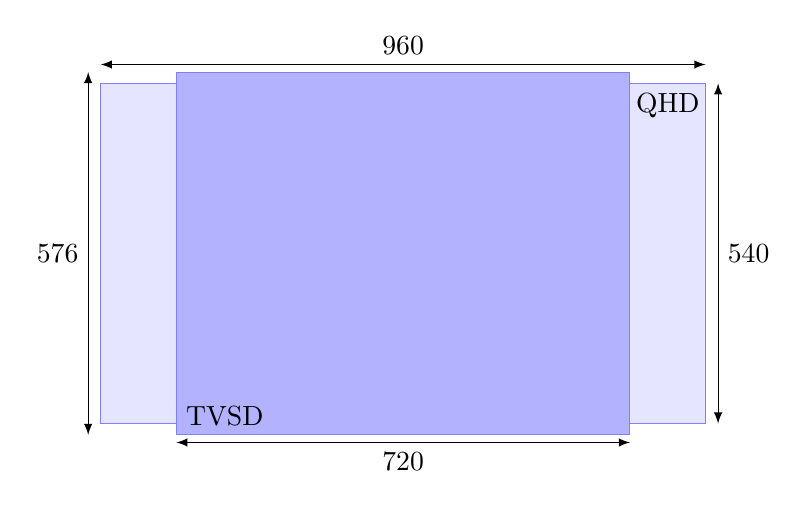
\begin{tikzpicture}[scale=.8]
\filldraw[draw=blue!50,fill=blue!10] (-4.8,-2.7) rectangle (4.8,2.7);
\filldraw[draw=blue!50,fill=blue!30] (-3.6,-2.88) rectangle (3.6,2.88);
% \draw[draw=blue!50] (-4.8,-2.7) rectangle (4.8,2.7);
\draw	(-3.6,-2.88) node[anchor=south west] {TVSD}
			(4.2,2.7) node[anchor=north] {QHD};

% QHD
\draw [<->,latex-latex] (5,-2.7) -- node[anchor=west] {540} (5,2.7);
\draw [<->,latex-latex] (-4.8,3) -- node[anchor=south] {960} (4.8,3);

% TVSD
\draw [<->,latex-latex] (-5,-2.88) -- node[anchor=east] {576} (-5,2.88);
\draw [<->,latex-latex] (-3.6,-3) -- node[anchor=north] {720} (3.6,-3);

\end{tikzpicture}
	\caption{Comparaison entre les définitions de QHD et de TVSD.}
	\label{fig:comparaisonTVSD-QHD}
\end{figure}


\subsubsection{Codage des contenus}
Suite à la création de contenus au format QHD, chacun est dégradé par le codeur de référence \avc~\cite{h264-jm}. C'est le même codeur que celui utilisé pour créer la base de séquences TVHD présentée à l'annexe~\ref{annex:base}. Nous avons déterminé sept débits de compression pour chaque séquence QHD. Ils sont présentés dans le tableau~\ref{tab:bitratesSD}. Parmi ces sept débits, deux sont retenus pour la comparaison avec la TVHD. Afin de les distinguer, ils sont graissés dans le tableau~\ref{tab:bitratesSD}. La sélection de ces débits résulte de la volonté de comparer la TVHD avec deux qualités distinctes et correspondant à une diffusion TVSD respectivement de qualité moyenne et bonne. Nous les appelons respectivement $Q_m$ et $Q_b$. De la même manière, sept débits de compression ont été définis pour chaque contenu TVHD. Les débits retenus sont présentés dans le tableau~\ref{tab:bitratesHD}.

\begin{table}[htbp]
\centering
\begin{tabular}{cc}\toprule
\strong{contenu} 						& \textbf{débit QHD (Mbps)}\\ \toprule
\emph{New Mobile \& Calendar}	& 1,2 ; 1,4 ; 1,7 ; \strong{1,8} ; 2,5 ; \strong{3} ; 4\\ \midrule
\emph{Parkrun}							& 4 ; 5 ; \strong{5,3} ; 7 ; 8 ; \strong{9} ; 12 \\ \midrule
\emph{Knightshields}					& 1 ; 1,4 ; \strong{1,6} ; 1,8 ; 2,5 ; \strong{3} ; 4\\ \midrule
\emph{Stockholm Pan}				& 0,6 ; 1 ; \strong{1,2} ; 1,4 ; \strong{1,8} ; 2,5 ; 6\\\bottomrule
\end{tabular}
\caption{Débits de compression pour chaque contenu QHD.}
\label{tab:bitratesSD}
\end{table}


\subsubsection{Évaluation subjective de la qualité des séquences}
La salle de test, les conditions d'expérimentation et le matériel sont les mêmes que pour l'évaluation subjective des séquences de la base de l'annexe~\ref{annex:base}. La figure~\ref{fig:MOSrateCodeurRefSD} présente les MOS en fonction du débit pour les quatre contenus SVT2002. Les MOS obtenus par les deux débits retenus pour correspondre à des qualités moyenne et bonne sont présentés dans le tableau~\ref{tab:bitratesSDQ60Q80}. Nous remarquons que les MOS obtenus ne correspondent pas exactement au terme choisi. Notamment, les séquences \emph{Parkrun} et \emph{Knighshields} obtiennent une valeur de $Q_m$ qui correspond plus à une qualité médiocre que moyenne. Ces MOS sont accompagnés de la différence entre ces deux qualités. Nous remarquons notamment que l'écart n'est pas significatif pour le contenu \emph{New Mobile \& Calendar}. En effet, la différence de qualité est faible compte tenu de la répartition des intervalles de confiance à 95\% obtenus lors de l'évaluation subjective de la base de l'annexe~\ref{annex:base}.

\begin{figure}[htbp]
\centering
\includegraphics[page=1, width=0.9\linewidth, trim= 70 50 90 70]{plot/debit-mosSD}
\caption{Notes de qualité en fonction du débit, exprimé en Mbps, obtenues pour le codeur de référence H.264 par les séquences QHD.}
\label{fig:MOSrateCodeurRefSD}
\end{figure}

\begin{table}[htbp]
\centering
\begin{tabular}{cDDp{0.1cm}c} \toprule
\multirow{2}{2.5cm}{\strong{contenu}} & \multicolumn{2}{c}{\strong{MOS}} & & \multirow{2}{1.5cm}{$Q_b - Q_m$}\tabularnewline
\cmidrule{2-3}
 & $Q_m$ & $Q_b$ & \tabularnewline \toprule
\emph{New Mobile \& Calendar}	& 49,7 & 56,1 & & 6,4\tabularnewline \midrule
\emph{Parkrun}							& 37,7 & 60,9 & & 23,2\tabularnewline \midrule
\emph{Knightshields}					& 36,3 & 55,2 & & 18,9\tabularnewline \midrule
\emph{Stockholm Pan}				& 50,9 & 65,3 & & 14,4\tabularnewline \bottomrule
\end{tabular}
\caption{MOS des séquences compressées à des débits correspondant à des qualités moyenne et bonne en TVSD, et différence entre les deux qualités.}
\label{tab:bitratesSDQ60Q80}
\end{table}


\subsubsection{Description du protocole d'évaluation}
Le protocole conçu dérive de la méthodologie comparative avec jugement catégoriel décrite dans la recommandation ITU-R BT.500-11~\cite{itu-bt500-11} et présentée section~\ref{ssec:Méthode_avec_échelle_dévaluation_par_catégorie}. Dans notre cas, l'attribution des deux séquence, une au format HD et l'autre au format SD, est aléatoire. De plus, après une première visualisation, l'observateur peut revoir les séquences autant de fois qu'il le désire, c'est le principe d'accès aléatoire présent dans la méthodologie SAMVIQ~\cite{ebu-samviq}. C'est la principale modification au protocole classique de comparaison. Elle se justifie par la précision accrue qu'elle apporte, comme nous l'avons montré dans la section précédente.

Après la présentation, l'observateur doit rapporter sa préférence entre les deux contenus. Pour cela, il utilise l'échelle de comparaison présentée dans le tableau~\ref{tab:compscale}. Les valeurs numériques relevées ne sont jamais indiquées à l'observateur. De plus, les termes utilisés dans l'échelle évitent les connotations qualitatives. Ainsi, l'observateur rapporte sa préférence globale, et pas seulement la qualité visuelle. Les tests effectués consistent donc en la comparaison d'un ensemble de sept séquences HD avec un ensemble de deux séquences SD. Une session est donc composée de 14 présentations par contenu. %Il faut bien saisir la complexité de la tâche demandée aux observateurs. Il est toujours délicat de comparer des choses très différentes. C'est pour cela que lors de la séance préparatoire, il leur était précisément indiqué de noter selon leur préférence globale. Néanmoins, cette complexité entraine une dispersion inévitable. C'est la raison pour laquelle les intervalles de confiance sont relativement élevés.

\begin{table}[htbp]
\centering
\begin{tabular}{cc}\toprule
\textbf{préférence} & \textbf{valeur} \\ \toprule
Je préfère beaucoup plus A que B & +3 \\ \midrule
Je préfère plus A que B & +2 \\ \midrule
Je préfère un peu plus A que B & +1 \\ \midrule
Je n'ai pas de préférence & 0 \\ \midrule
Je préfère un peu moins A que B & --1 \\ \midrule
Je préfère moins A que B & --2 \\ \midrule
Je préfère beaucoup moins A que B & --3 \\ \bottomrule
\end{tabular}
\caption{Échelle de comparaison utilisée pour les tests de préférence entre télévision standard et télévision haute définition.}
\label{tab:compscale}
\end{table}


\subsection{Effets opposés de la taille de l'écran et des distorsions}
Pour évaluer la préférence moyenne entre TVHD et TVSD par rapport à leur différence de qualité, nous l'évaluons en fonction du $\Delta$MOS, calculé comme la différence entre le MOS de la TVHD et le MOS de la TVSD, pour chaque débit. Pour mieux comprendre le sens d'une telle représentation, la figure ~\ref{fig:lectureCourbesHDvsSD} délimite l'espace entre quatre quadrants, chacun ayant une signification précise. Les droites en pointillés sont particulièrement intéressantes. La verticale représente l'égalité des qualités TVHD et TVSD. L'horizontale représente l'isopréférence de l'observateur moyen entre TVHD et TVSD.

\begin{figure}[htbp]
\centering
\begin{tikzpicture}[scale=2.5]% comment lire les courbes HDvsSD

% \begin{tikzpicture}[scale=2]
	% The graphic
	\filldraw[draw=red!30,fill=red!30] (0,0) rectangle (2.5,1);
	\filldraw[draw=green!30,fill=green!30] (0,0) rectangle (-2.5,1);
	\filldraw[draw=blue!30,fill=blue!30] (0,0) rectangle (2.5,-1);
	\filldraw[draw=yellow!30,fill=yellow!30] (0,0) rectangle (-2.5,-1);

 	\draw[->] (-2.5,-1) -- (2.6,-1) node[below] {$\Delta$MOS} coordinate(x axis);
 	\draw[->] (-2.5,-1) -- (-2.5,1.2) node[above, text width=2cm, text centered] {préférence moyenne} coordinate(y axis);

	\draw (-2.6,0) node{0};
	\draw (0,-1.1) node{0};
	\draw[dotted] (-2.5,0) -- (2.5,0);
	\draw[dotted] (0,1) -- (0,-1);

	\draw (2.5,0.9) node[left] {HD préférée};
	\draw (2.5,0.7) node[left] {$MOS_{HD} > MOS_{SD}$};
	\draw (-2.5,0.9) node[right] {HD préférée};
	\draw (-2.5,0.7) node[right] {$MOS_{HD} < MOS_{SD}$};
	\draw (2.5,-0.9) node[left] {SD préférée};
	\draw (2.5,-0.7) node[left] {$MOS_{HD} > MOS_{SD}$};
	\draw (-2.5,-0.9) node[right] {SD préférée};
	\draw (-2.5,-0.7) node[right] {$MOS_{HD} < MOS_{SD}$};

	\draw (2.5,0.05) node[left, blue]{isopréférence};% (image size)};
	\draw (0,0) node[above, blue, rotate=90]{$MOS_{HD} = MOS_{SD}$};% (distortions)};
% \end{tikzpicture}
\end{tikzpicture}
\caption{Lecture des courbes de préférence entre TVHD et TVSD en fonction du $\Delta$MOS.}
\label{fig:lectureCourbesHDvsSD}
\end{figure}

% FIXME essayer de les placer sur la même page !

\begin{figure}[htbp]
\centering
\subfloat{\includegraphics[page=1, width=0.48\linewidth, trim= 70 50 90 70]{plot/HDvsSD-LCD}}\hfill
\subfloat{\includegraphics[page=2, width=0.48\linewidth, trim= 70 50 90 70]{plot/HDvsSD-LCD}}\\
\subfloat{\includegraphics[page=3, width=0.48\linewidth, trim= 70 50 90 70]{plot/HDvsSD-LCD}}\hfill
\subfloat{\includegraphics[page=4, width=0.48\linewidth, trim= 70 50 90 70]{plot/HDvsSD-LCD}}\\
\caption{Préférence moyenne entre TVHD et TVSD en fonction du $\Delta$MOS pour quatre séquences SVT2002.}
\label{fig:HDvsSD-LCD}
\end{figure}

La figure~\ref{fig:HDvsSD-LCD} présente ces courbes pour les quatre contenus SVT2002. %De plus, elle présente les intervalles de confiance à 95\% calculés sur la préférence et sur les MOS.
Les flèches indiquent les valeurs $\Delta$MOS$_0$, prises à l'équilibre de la préférence entre TVHD et TVSD pour chaque contenu. Si $\Delta$MOS$_0$ est négatif, cela signifie que quand l'observateur moyen n'a pas de préférence entre les deux séquences, c'est celle au format HD qui a la moins bonne qualité. Le tableau~\ref{tab:DeltaMOS-MOShd-LCD} contient les valeurs de $\Delta$MOS$_0$ pour tous les contenus ainsi que le MOS de la version TVHD en ces points. Ce MOS$_{\HD}$ correspond à la qualité à partir de laquelle l'observateur moyen préfère la TVHD.%Les valeurs au passage à zéro ont été obtenues par interpolation linéaire.

\begin{table}[htbp]
\centering
\begin{tabular}{ccccc}\toprule
\multirow{2}{2.5cm}{\strong{contenu}} & \multicolumn{2}{c}{$Q_m$} & \multicolumn{2}{c}{$Q_b$}\tabularnewline
\cmidrule{2-5}
													& $\Delta$MOS$_0$ 	& MOS$_{\HD}$ 	& $\Delta$MOS$_0$ 	& MOS$_{\HD}$\\ \toprule
\emph{New Mobile \& Calendar}	& --18,0 						& 31,7					& --12,50						& 43,6\\ \midrule
\emph{Parkrun}							& --8,0 							& 29,6					& --18,0						& 42,9\\ \midrule
\emph{Knightshields}					& --1,8 							& 34,5					& 0								& 55,2\\ \midrule
\emph{Stockholm Pan}				& --12,0 						& 38,9					& --17.6						& 47,7\\ \bottomrule
\end{tabular}
\caption{$\Delta$MOS$_0$ et MOS$_{\HD}$ pour les qualités $Q_m$ et $Q_b$, et les quatre contenus SVT2002.}
\label{tab:DeltaMOS-MOShd-LCD}
\end{table}

Au vu du faible écart entre $Q_m$ et $Q_b$ pour le contenu \emph{New Mobile \& Calendar}, nous l'avons écarté de l'analyse. En effet, cela traduit le fait que l'observateur moyen fait une distinction de qualité insuffisante entre les deux séquences. La conséquence est que les préférences et les $\Delta$MOS sont proches les uns des autres.

Nous remarquons tout d'abord que lorsque la qualité de la TVHD décroit, la TVSD finit par être préférée à la TVHD, ce qui est le comportement attendu. En effet, à qualité TVSD constante, plus les dégradations introduites dans la TVHD vont gêner l'observateur et plus il va préférer l'autre version disponible.

Ensuite, les valeurs de $\Delta$MOS$_0$ sont toutes négatives ou nulles. Cela signifie que quand les observateurs n'ont pas de préférence particulière pour l'un ou l'autre des formats, la qualité intrinsèque de la TVSD est supérieure. De plus, cette supériorité est significative pour tous les contenus sauf \emph{Knightshields}. Cette différence de qualité en faveur de  la TVSD est compensée par la taille de l'image en TVHD. C'est ce que nous appelons l'\emph{effet grand écran}. L'observateur moyen est prêt à perdre un peu de qualité intrinsèque s'il peut bénéficier d'une image plus grande. La TVHD peut alors présenter plus de dégradations et obtenir la même préférence que la TVSD.

Ceci est d'autant plus vrai que $\Delta$MOS$_0$ est négatif. Or en dehors de la séquence \emph{New Mobile \& Calendar} que nous avons écarté, nous avons toujours $\Delta$MOS$_0(Q_m) > \Delta$MOS$_0(Q_b)$. Ainsi, quand la TVHD est comparée à une TVSD de bonne qualité $Q_b$, l'effet grand écran est prédominant. L'observateur moyen tire avantage de la taille de l'écran pour profiter pleinement de la TVHD.

Par contre, quand la TVHD est comparée à une TVSD de qualité moyenne $Q_m$, cet effet décroit. Les valeurs de $\Delta$MOS$_0$ croissent significativement, sauf pour \emph{Knightshields} pour qui les valeurs ne sont pas significativement différentes. Ainsi, quand les observateurs n'ont pas de préférence particulière entre les qualités de la TVHD et de la TVSD, leurs qualités intrinsèques sont plus proches. Cela signifie que l'effet grand écran perd ici de son influence au profit de l'impact des dégradations même de la séquence. Celle-ci est tellement dégradée que l'observateur moyen tend à préférer la TVSD car subir des distorsions sur une petite image est moins gênant que sur une grande. Ici, l'effet des dégradations est prédominant dans l'élaboration de la préférence de l'observateur.

Ceci fournit une information de première importance pour les diffuseurs de télévision haute définition. La TVHD doit être de qualité significativement supérieure afin de tirer tout le bénéfice de l'effet grand écran et non pas le transformer en déficit. %La qualité visuelle en TVHD doit donc être assurée pour que les usagers trouve un intérêt au passage à cette nouvelle technologie.


\subsection{Conclusion}
Cette section a permis de déterminer la préférence de l'observateur moyen entre la télévision haute définition et la télévision standard. L'étude menée a consisté à comparer directement les deux formats lors de tests subjectifs. Pour cela, un protocole et une méthodologie de visualisation simultanée des deux formats ont été conçus. Ces tests ont donc été réalisés avec d'un côté le respect maximal des recommandations en terme de conditions expérimentales, et de l'autre, la nécessité de définir de nouvelles propriétés à des tests sans précédent dans la littérature.

L'enseignement de cette étude est que l'observateur moyen doit composer avec deux effets contradictoires. D'un côté, il peut bénéficier d'une plus grande image et donc d'une meilleure qualité visuelle. De l'autre, il peut subir des dégradations importantes dues au codage \avc, ce qui fait chuter cette même qualité visuelle. Afin de la conserver à un haut niveau et donc de satisfaire l'observateur, un service de TVHD doit donc assurer une qualité visuelle de haut niveau. L'exploitation intéressante de la haute définition doit être liée à une faible quantité de dégradations visibles.


\section{Impact de l'affichage sur la qualité} \label{sec:Études_Impact_Affichage_Qualité}
La transition vers la haute définition s'accompagne d'une modification des techniques d'affichage. Cela a évidemment un impact sur la qualité d'image que nous cherchons à évaluer. Nous nous intéressons à l'effet lié aux technologies CRT et LCD, qui sont techniquement très différentes. Les avantages du LCD sont son encombrement réduit et sa plus grande gamme de luminosité. Cependant, le temps de réponse de l'écran et les défauts de restitution des zones sombres et du mouvement ont un impact important sur la perception de la qualité. Le mouvement sur un écran LCD est accompagné d'un flou caractéristique. Celui-ci est dû à la manière dont l'image est affichée. Dans la technologie CRT, une image est affichée par un balayage pixel par pixel. Ainsi, l'image n'est pas maintenue entre deux balayages successifs. La persistance rétinienne permet de créer un mouvement apparent grâce à la grande vitesse de balayage. Par contre,  sur un écran LCD, les pixels sont affichés tous ensemble et l'image est maintenue affichée en attendant la suivante. Or, pour un contenu en mouvement, l'\oe il humain a naturellement tendance à le suivre au cours du temps. Ce suivi, combiné au maintien de l'image sur l'écran, entraine l'intégration temporelle de l'objet sur la rétine, ce que l'observateur ressent comme du flou. Les figures~\ref{fig:integrationLCD} et~\ref{fig:integrationCRT} illustrent ces principes. Ce défaut majeur a été étudié par Sylvain Tourancheau~\cite{tourancheau-vpqm2007, tourancheau-icip2007}. Il a notamment montré l'impact de la définition sur la différence de perception de la qualité entre un écran CRT et un écran LCD.

\begin{figure}[htbp]
	\centering
	\subfloat[\label{fig:integrationLCD} Perception d'un objet en mouvement avec un écran LCD.]{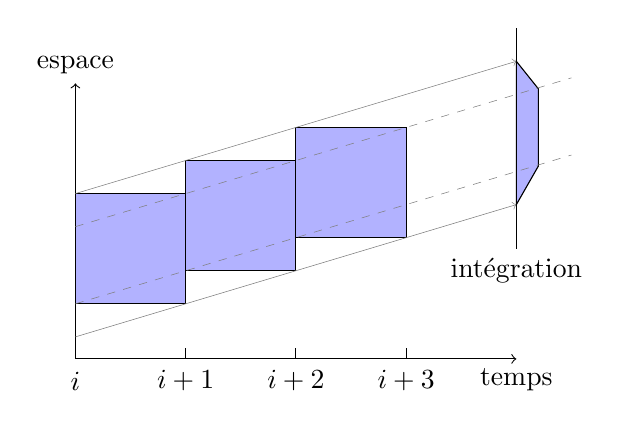
\begin{tikzpicture}[scale=1.4]\filldraw[fill=blue!30] (0,0.5) rectangle (1,1.5);
\filldraw[fill=blue!30] (1,0.8) rectangle (2,1.8);
\filldraw[fill=blue!30] (2,1.1) rectangle (3,2.1);

\draw[->] (0,0) -- (4,0) node[below] {temps} coordinate(x axis);
\draw[->] (0,0) -- (0,2.5) node[above] {espace} coordinate(y axis);
\draw (0, -0.2) node{$i$};
\draw (1,-0.2) node{$i+1$};
\draw (1,0) -- (1,0.1);
\draw (2,-0.2) node{$i+2$};
\draw (2,0) -- (2,0.1);
\draw (3,-0.2) node{$i+3$};
\draw (3,0) -- (3,0.1);

\draw[help lines,->] (0,1.5) -- (4,2.7);
\draw[help lines,->] (0,0.2) -- (4,1.4);

\filldraw[fill=blue!30] (4,2.7) -- (4,1.4) -- (4.2,1.75) -- (4.2,2.45) -- cycle;
\draw[help lines,dashed] (0,0.5) -- (4.5,1.85);
\draw[help lines,dashed] (0,1.2) -- (4.5,2.55);

\draw (4,3) -- (4,1) node[below]{intégration};
\end{tikzpicture}}\hfill
	\subfloat[\label{fig:integrationCRT} Perception d'un objet en mouvement avec un écran CRT.]{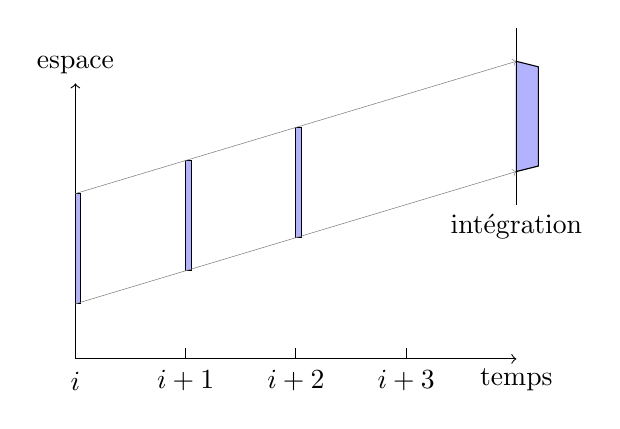
\begin{tikzpicture}[scale=1.4]\filldraw[fill=blue!30] (0,0.5) rectangle (0.05,1.5);
\filldraw[fill=blue!30] (1,0.8) rectangle (1.05,1.8);
\filldraw[fill=blue!30] (2,1.1) rectangle (2.05,2.1);

\draw[->] (0,0) -- (4,0) node[below] {temps} coordinate(x axis);
\draw[->] (0,0) -- (0,2.5) node[above] {espace} coordinate(y axis);
\draw (0, -0.2) node{$i$};
\draw (1,-0.2) node{$i+1$};
\draw (1,0) -- (1,0.1);
\draw (2,-0.2) node{$i+2$};
\draw (2,0) -- (2,0.1);
\draw (3,-0.2) node{$i+3$};
\draw (3,0) -- (3,0.1);

\draw[help lines,->] (0,1.5) -- (4,2.7);
\draw[help lines,->] (0,0.5) -- (4,1.7);

\filldraw[fill=blue!30] (4,2.7) -- (4,1.7) -- (4.2,1.75) -- (4.2,2.65) -- cycle;
\draw (4,3) -- (4,1.4) node[below]{intégration};
\end{tikzpicture}}\\
	\caption{Comparaison de la perception d'un objet en mouvement avec un écran LCD et CRT.}
\end{figure}

Le second effet est lié au type de méthodologie utilisée dans le redimensionnement d'image. En effet, alors que les écrans de TVHD ont tous une définition supérieure à celle de la TVSD, ils devront, pendant une période, être capable d'afficher des images dans les deux définitions. Or, ce traitement a un cout en termes de qualité d'image et nous voulons mesurer cette perte. Dans le but d'évaluer l'impact du type de technologie d'affichage, des tests ont été réalisés à la fois sur l'écran LCD et sur l'écran CRT. Parmi ceux-ci, nous en avons effectué sur des séquences de définition QHD, QHD redimensionnée et TVHD afin d'évaluer l'impact de l'adaptation de l'image à une certaine définition.


\subsection{Impact du type de technologie d'affichage} \label{ssec:impactTechnoAffichage}
La figure~\ref{fig:nuageMOSCRTLCD} présente les MOS mesurés sur écran LCD en fonction des MOS mesurés sur écran CRT pour 96 séquences de TVHD. La droite pointillée correspond à l'égalité des MOS. Le coefficient de corrélation linéaire entre les deux ensembles de données est de 0,950. Cela montre la bonne cohérence des deux évaluations. Il existe donc une relation forte entre les deux ensembles de MOS. Il est possible de définir une fonction de transformation de l'un à l'autre comme l'a fait Tourancheau~\cite{tourancheau-vpqm2007}. Cependant, le nuage de points montre une nette supériorité pour le CRT. En effet, les qualités mesurées sur le CRT sont, à quelques exceptions près, toujours supérieures à celles mesurées sur le LCD. La racine carrée de l'erreur quadratique moyenne reqm par contenu est présentée dans le tableau~\ref{tab:diffMOS}.

\begin{figure}[htbp]
	\centering
	\begin{tikzpicture}[only marks, scale=0.07]
		\pgfsetplotmarksize{1.5cm}
		\draw plot[mark=+] file {plot/chap2/MOS-LCD-CRT.txt};
		\draw[->] (0,0) -- node[below=0.5cm] {MOS sur CRT} (95,0);
		\draw[->] (0,0) -- node[above=0.7cm, sloped] {MOS sur LCD} (0,95) ;
		\foreach \x in {0,15,30,45,60,75,90} \draw (\x,1) -- (\x,-1) node[anchor=north] {\x};
		\foreach \y in {0,15,30,45,60,75,90} \draw (1,\y) -- (-1,\y) node[anchor=east] {\y};
		\draw[dotted] (0,0) -- (90,90);
	\end{tikzpicture}
	\caption{MOS LCD en fonction des MOS CRT pour 96 séquences.}
	\label{fig:nuageMOSCRTLCD}
\end{figure}

\begin{table}[htbp]
\centering
\begin{tabular}{cc}\toprule
\textbf{séquence}						& \textbf{reqm}	\\ \toprule
\emph{New Mobile \& Calendar}	& 12,47	\\\midrule
\emph{Parkrun}							& 10,02	\\\midrule
\emph{Knightshields}					& 11,69	\\\midrule
\emph{Stockholm Pan}				& 8,60		\\\midrule
\emph{Concert}							& 12,07	\\\midrule
\emph{Foot}								& 16,38	\\\midrule
\emph{Movie}								& 18,49	\\\midrule
\emph{Voile}								& 14,87	\\\midrule
\emph{Crédits}							& 16,68	\\\midrule
\emph{Golf}									&  9,72		\\\midrule
\emph{Show}								& 14,99	\\\midrule
\emph{Standing}							& 16,17	\\\bottomrule
\end{tabular}
\caption{Racine carrée de l'erreur quadratique moyenne entre les qualités subjectives mesurées sur écran CRT et sur écran LCD pour chaque séquence SVT2002 et Euro1080.}
\label{tab:diffMOS}
\end{table}

Les plus fortes valeurs correspondent aux contenus \emph{Foot}, \emph{Movie}, \emph{Crédits} et \emph{Standing}. Les plus faibles correspondent à \emph{Stockholm Pan} et \emph{Golf}. Les origines de ces valeurs extrêmes sont variées. Foot se distingue par un fort mouvement d'ensemble dans la séquence. Il en est de même pour \emph{Crédits} où, en plus, du texte défile de bas en haut. Or, nous savons que le flou de mouvement est un des défauts majeurs de l'affichage LCD. Par contre, \emph{Movie} est très statique et présente un concert dans une cathédrale filmé de haut. \emph{Standing} est également très statique et ne présente qu'un orateur en plan rapproché poitrine. L'attention de l'observateur, non captée par une scène à si faible contenu informatif, se détourne rapidement pour détecter les dégradations, notamment dans les nombreuses zones sombres présentes autour de l'orateur. Le rendu de ces zones sombres est également un défaut connu de la technologie LCD. À l'opposé, \emph{Stockholm Pan} et \emph{Golf} sont des séquences très statiques et lumineuses. La première est un panorama de la ville de Stockholm en pleine journée. La seconde est un plan sur des joueurs de golf avec un fort ensoleillement. Avec ce type de contenu, l'écran LCD fournit une bonne qualité d'image.

Ces résultats illustrent donc l'impact de la technologie d'affichage utilisée. Cela a son importance et les constructeurs d'écran l'ont bien compris, puisque tous les écrans actuels incorporent de nombreux post-traitements, toujours en nombre croissant. De plus, cette étude confirme les résultats de celle de l'ITU~\cite{itu-crtlcd} présentée en \ref{ssec:itu}. Cependant cette fois-ci, nous utilisons deux écrans de résolution native 1920\texttimes1080, ce qui n'introduit pas de biais supplémentaire.


\subsection{Impact de l'adaptation de l'image à une définition supérieure}
Lors de l'affichage d'une image de TVSD sur un écran de TVHD, une technique de sur-échantil\-lon\-nage doit être utilisée. Celle-ci engendre des dégradations visibles. Pour déterminer la perte de qualité provoquée, nous avons évalué la qualité de séquences sur-échantillonnées. Les séquences au format QHD crées dans la section précédente ont subit un tel traitement. Le résultat de ce traitement est nommé TVHD'. L'algorithme Lanczos3, très utilisé et réputé dans le domaine du redimensionnement, est appliqué sur ces 28 séquences et les quatre contenus correspondants. Cette méthode d'interpolation est définie sur une fenêtre comme un produit de fonctions sinus cardinal normalisées. Le noyau obtenu est utilisé pour convoluer l'image à retailler. L'approximation effectuée est fonction de la taille de la fenêtre utilisée. La figure~\ref{fig:TVHD2QHD2TVHDp} présente le schéma de création de chaque type de séquence à partir de de la source TVHD.

\begin{figure}[htbp]
	\centering
	\begin{tikzpicture}[text centered, text width=3em, node distance = 2.5cm]
	\node (tvhd) {TVHD};
	\node[action, right of=tvhd, text width=5em] (filtre) {filtre demi-bande};
	\node[action, right of=filtre] (down) {$\downarrow$ 2};
	\node[right of=down] (qhd) {QHD};
	\node[action, right of=qhd, text width=5em] (up) {$\uparrow$ 2 Lanczos3};
	\node[right of=up, text width=3.2em] (tvhdp) {TVHD'};
	\path [fleche] (tvhd) -- (filtre);
	\path [fleche] (filtre) -- (down);
	\path [fleche] (down) -- (qhd);
	\path [fleche] (qhd) -- (up);
	\path [fleche] (up) -- (tvhdp);
	\end{tikzpicture}
	\caption{Schéma de création des séquences QHD et TVHD' à partir des séquences TVHD.}%
	\label{fig:TVHD2QHD2TVHDp}%
\end{figure}

La qualité des séquences TVHD' est mesurée dans les mêmes conditions d'expérimentation que pour les séquences de TVHD et de QHD. Les figures~\ref{fig:HD-SDup-LCD} et~\ref{fig:SD-SDup-LCD} présentent respectivement les MOS des séquences de TVHD' en fonction des MOS des séquences de QHD et des MOS des séquences de TVHD originales mesurés sur un écran LCD. Les figures~\ref{fig:HD-SDup-CRT} et~\ref{fig:SD-SDup-CRT} présentent respectivement les MOS des séquences de TVHD' en fonction des MOS des séquences de QHD et des MOS des séquences de TVHD originales mesurés sur un écran CRT.

\begin{figure}[htbp]
	\centering
\subfloat[\label{fig:HD-SDup-LCD}MOS des séquences de TVHD' en fonction des MOS des séquences de TVHD sur LCD.]{
	\begin{tikzpicture}[only marks, scale=0.09]
		\pgfsetplotmarksize{1cm}
		\draw plot[mark=+] file {plot/chap2/HD-SDup-LCD.txt};
		\draw[->] (20,20) -- node[below=0.5cm] {MOS TVHD} (85,20);
		\draw[->] (20,20) -- node[above=0.7cm, sloped] {MOS TVHD'} (20,85) ;
		\foreach \x in {20,40,60,80} \draw (\x,21) -- (\x,19) node[anchor=north] {\x};
		\foreach \y in {20,40,60,80} \draw (21,\y) -- (19,\y) node[anchor=east] {\y};
		\draw[dotted] (20,20) -- (80,80);
	\end{tikzpicture}}\hfill
\subfloat[\label{fig:SD-SDup-LCD}MOS des séquences de TVHD' en fonction des MOS des séquences de QHD sur LCD.]{
	\begin{tikzpicture}[only marks, scale=0.09]
		\pgfsetplotmarksize{1cm}
		\draw plot[mark=+] file {plot/chap2/SD-SDup-LCD.txt};
		\draw[->] (20,20) -- node[below=0.5cm] {MOS QHD} (85,20);
		\draw[->] (20,20) -- node[above=0.7cm, sloped] {MOS TVHD'} (20,85) ;
		\foreach \x in {20,40,60,80} \draw (\x,21) -- (\x,19) node[anchor=north] {\x};
		\foreach \y in {20,40,60,80} \draw (21,\y) -- (19,\y) node[anchor=east] {\y};
		\draw[dotted] (20,20) -- (80,80);
	\end{tikzpicture}}\\
	\subfloat[\label{fig:HD-SDup-CRT}MOS des séquences de TVHD' en fonction des MOS des séquences de TVHD sur CRT.]{
	\begin{tikzpicture}[only marks, scale=0.09]
		\pgfsetplotmarksize{1cm}
		\draw plot[mark=+] file {plot/chap2/HD-SDup-CRT.txt};
		\draw[->] (20,20) -- node[below=0.5cm] {MOS TVHD} (85,20);
		\draw[->] (20,20) -- node[above=0.7cm, sloped] {MOS TVHD'} (20,85) ;
		\foreach \x in {20,40,60,80} \draw (\x,21) -- (\x,19) node[anchor=north] {\x};
		\foreach \y in {20,40,60,80} \draw (21,\y) -- (19,\y) node[anchor=east] {\y};
		\draw[dotted] (20,20) -- (80,80);
	\end{tikzpicture}}\hfill
	\subfloat[\label{fig:SD-SDup-CRT}MOS des séquences de TVHD' en fonction des MOS des séquences de QHD sur CRT.]{
	\begin{tikzpicture}[only marks, scale=0.09]
		\pgfsetplotmarksize{1cm}
		\draw plot[mark=+] file {plot/chap2/SD-SDup-CRT.txt};
		\draw[->] (20,20) -- node[below=0.5cm] {MOS QHD} (85,20);
		\draw[->] (20,20) -- node[above=0.7cm, sloped] {MOS TVHD'} (20,85) ;
		\foreach \x in {20,40,60,80} \draw (\x,21) -- (\x,19) node[anchor=north] {\x};
		\foreach \y in {20,40,60,80} \draw (21,\y) -- (19,\y) node[anchor=east] {\y};
		\draw[dotted] (20,20) -- (80,80);
	\end{tikzpicture}}\\
	\caption{Comparaison des MOS des séquences QHD, TVHD' et TVHD sur un écran CRT et un écran LCD.}
\end{figure}

Il est clair que l'adaptation de l'image à une définition supérieure a un impact sur la qualité perçue. Dans les quatre comparaisons, les séquences ayant subi un redimensionnement ont une qualité nettement inférieure. Il est logique que la comparaison avec la TVHD soit à l'avantage de celle-ci. Le traitement ne peut retrouver la qualité originale perdue dans le sous-échantil\-lon\-nage. La perte est sensible, surtout dans les hautes qualités. La différence est moins prononcée dans les qualités basses, ce qui est dû aux dégradations. Celles-ci sont alors particulièrement visibles et gênantes et l'impact du redimensionnement y est moins important. Néanmoins, les applications de TVHD situent leur gamme dans les hautes et très hautes qualités, c'est donc dans ces gammes qu'il faut être performant.

Sur écran LCD, les MOS des séquences de TVHD et ceux des séquences de TVHD' montrent un coefficient de corrélation linéaire de 0,940 et une racine carrée de l'erreur quadratique moyenne de 13,73. Malgré la nette différence en faveur de la TVHD, les MOS conservent une relation forte. Sur écran CRT, le coefficient de corrélation chute à 0,839 et la racine carrée de l'erreur quadratique moyenne vaut 16,50. La relation est beaucoup moins importante et l'erreur s'accroit. Nous savons que les MOS mesurés sur CRT sont plus élevés que sur LCD. Si la corrélation chute sur cet écran, cela renforce l'importance de l'écart entre TVHD et TVHD'.

Plus étonnant, la différence de qualité entre la version TVHD' et la version QHD est approximativement du même ordre que celle entre la version TVHD' et la version de TVHD. En effet la racine carrée de l'erreur quadratique moyenne est de 12,80 sur l'écran LCD et de 14,61 sur l'écran CRT. Dans ce cas, bien que les observateurs bénéficient d'une grande image, l'impact du traitement de redimensionnement est tel qu'ils attribuent une meilleure qualité à la version non traitée. De plus, sur écran LCD, les MOS des séquences de QHD et ceux des séquences de TVHD' produisent un coefficient de corrélation linéaire de 0,960. Sur écran CRT, il chute à 0,906. Bien que moins importante, nous constatons la même chute que pour la comparaison entre TVHD et TVHD'.

Pour les services de TVHD, cela signifie qu'un écran ne gagne pas en qualité à étirer l'image à la taille de la dalle. Néanmoins, les technologies d'affichage moderne incluent des traitements permettant d'atténuer les dégradations dues à cet étirement. Nous n'en avons pas évalué, mais il nous apparait ici comme évident que ce type de traitements est indispensable.


\subsection{Conclusion} % TODO réflexion de fond à mener
Nous tirons deux conclusions majeures de cette section. Tout d'abord, nous avons montré la différence de qualités visuelles mesurées sur deux écrans de différentes technologies. Les MOS mesurés sur un écran de type CRT sont significativement supérieurs à ceux mesurés sur un écran de type LCD. Cependant, cette conclusion doit être relativisée par le fait que l'écran CRT était un matériel professionnel et que l'écran LCD était utilisé sans aucun post-traitement d'affichage. %Le but est donc uniquement de comparer les technologies d'affichage.

Nous nous sommes aussi intéressés à l'impact du redimensionnement d'image pour l'affichage. Celui-ci est couramment utilisé dans les téléviseurs modernes. Ce type de traitement a évidemment un impact négatif sur la qualité comparée à la qualité originale de la TVHD. Il est plus surprenant de constater qu'un écart important est mesuré quand ces séquences redimensionnées sont comparées avec les séquences de définition standard. Bien que permettant un effet grand écran artificiel, cette pratique est destructrice de qualité, et son utilisation seule n'apporte rien à l'utilisateur final.


\section{Conclusion}
Plusieurs aspects de la qualité visuelle en télévision haute définition ont été étudiés. Nous avons d'abord définit clairement la notion de qualité d'usage que nous avons réduit à la qualité visuelle. Trois aspects ont par la suite été développés. Concernant l'impact de la méthodologie d’évaluation subjective de la qualité, nous avons montré :
\begin{itemize}
\item que les méthodologies ACR et SAMVIQ ne fournissent pas des mesures de qualités similaires en TVHD, le choix de l'une ou l'autre doit donc être fait en connaissance de cause ;
\item que la taille de l'image, et donc celle du champ visuel excité, a une influence sur l'évaluation de qualité, ce qui explique une chute du coefficient de corrélation entre les évaluations produites par les méthodologies ACR et SAMVIQ en TVHD ;
\item qu'à nombre d'observateurs identique, la méthodologie SAMVIQ fournit des MOS de plus grande précision que la méthodologie ACR.
\end{itemize}

Dans la suite de nos travaux, la méthodologie SAMVIQ sera privilégiée. Elle a ainsi permis d'évaluer la qualité sur une base importante de 192 séquences TVHD. Les résultats de cette évaluation sont utilisés dans une étude de préférence entre la télévision haute définition et télévision standard. Dans cette étude, nous avons :
\begin{itemize}
\item conçu une méthodologie de comparaison visuelle de contenus à plusieurs définitions ;
\item identifié deux effets contradictoires avec lesquels l'observateur moyen doit composer lorsqu'il passe de la TVSD à TVHD, à savoir la taille de l'écran et la quantité de dégradations contenue ;
\item déterminé les zones d'influence de ces deux effets ;
\item montré que le gain en qualité visuelle de la télévision haute définition est directement lié à une faible quantité de dégradations perçues.
\end{itemize}

Enfin, nous avons évalué l'impact de l'affichage sur la qualité. Pour cela, nous avons d'une part effectué des tests à la fois sur écran LCD et sur écran CRT. D'autre part, nous avons évalué des séquences vidéos à différentes définitions, ayant subit pour cela un redimensionnement de taille. Ceci a permis :
\begin{itemize}
\item de montrer que la différence de technologie d'affichage introduit un biais de qualité en faveur de l'écran CRT ;
\item de constater que les techniques de redimensionnement d'image provoquent des pertes de qualité sensibles.
\end{itemize}

L'ensemble de ces contributions nous a permis de mieux comprendre l'impact de la télévision haute définition sur la qualité visuelle. Les changements que cette nouvelle technologie implique sont nombreux et nécessitent des précautions quant à leur utilisation par les usagers. Ceux-ci doivent bénéficier d'une qualité visuelle sensiblement supérieure afin d'assurer le succès du système. Dans cette optique, il peut être intéressant de connaitre l'impact des dégradations de type codage sur la qualité visuelle. C'est l'objet du prochain chapitre.


\ornementChapitre
